\documentclass [xcolor=svgnames, t] {beamer} 
\usepackage[utf8]{inputenc}
\usepackage{booktabs, comment} 
\usepackage[absolute, overlay]{textpos} 
\usepackage{pgfpages}
\usepackage[font=footnotesize]{caption}
\useoutertheme{infolines} 

\AtBeginSection[]{
  \begin{frame}
  \vfill
  \centering
  \begin{beamercolorbox}[sep=8pt,center,shadow=true,rounded=true]{title}
    \usebeamerfont{title}\insertsectionhead\par%
  \end{beamercolorbox}
  \vfill
  \end{frame}
}


%\definecolor{brownbrown}{RGB}{56, 28, 0}
%\definecolor{brownred}{RGB}{228, 0, 43}

%\setbeamercolor{title in head/foot}{bg=brownred, fg=brownbrown}
%\setbeamercolor{author in head/foot}{bg=myuniversity}
\setbeamertemplate{page number in head/foot}{}
\usepackage{csquotes}


\usepackage{amsmath}
\usepackage[makeroom]{cancel}
\usepackage[absolute,overlay]{textpos}
\usepackage{tcolorbox}

%\usepackage{textpos}

\usepackage{tikz}

\usepackage{media9} 

\usetheme{Madrid}
%\definecolor{myuniversity}{RGB}{56, 28, 0}
%\usecolortheme[named=myuniversity]{structure}



\title[HEC-RAS]{Introducci\'on a HEC-RAS}
\subtitle{Introducci\'on al analisis de flujo a superficie libre usando HEC-RAS}
\institute[]{Departamento de Ingenier\'ia Civil y Agr\'icola\\ Facultad de Ingenier\'ia  \\Universidad Nacional de Colombia - Sede Bogot\'a}
\titlegraphic{
\includegraphics[height=2.0cm]{escudoUnal.png}}
\author[LAM]{Luis Alejandro Morales \\ \href{https://lamhydro.github.io}{https://lamhydro.github.io}}


%\institute[]{Department of Earth, Environmental, and Planetary Sciences  \\Brown University}
\date{\today}


\addtobeamertemplate{navigation symbols}{}{%
    \usebeamerfont{footline}%
    \usebeamercolor[fg]{footline}%
    \hspace{1em}%
    \insertframenumber/\inserttotalframenumber
}

\begin{document}
\begin{frame}
\maketitle
\end{frame}

%%%%%%%%%%%%%%%%%%%%%%%%%%%%
\logo{\vspace{-0.2cm}
\includegraphics[height=0.8cm]{escudoUnal.png}~%
}
%%%%%%%%%%%%%%%%%%%%%%%%%%


\begin{frame}
\frametitle{Table of Contents}
\tableofcontents
\end{frame}

\section{Introducci\'on}
\begin{frame}{Generalidades}
\begin{block}{Generalidades}
Existen diferentes herramientas computaciones para el an\'alisis di\'amico del flujo, que dependiendo de su especialidad, se tiene:
\begin{itemize}
    \item \emph{HEC-RAS}: An\'alisis de flujo a superficie libre en canales.
    \item \emph{EPASWMM}: An\'alisis del flujo en sistemas de alcantirallo pluvial o sanitario.
    \item \emph{QUAL2E}: Calidad del agua en rios. 
\end{itemize}
Depenpendiendo de la dimensi\'on espacial de analisis de flujo:

\begin{itemize}
    \item \emph{Modelos 1D}: MIKE11 y HEC-RAS
    \item \emph{Modelos 2D}: FLOW-2D, iRIC, TELEMAC, IBER, HEC-RAS
    \item \emph{Modelos 3D}: DELF3D
\end{itemize}
\end{block}
\end{frame} 


\begin{frame}{HEC-RAS}
\begin{block}{HEC-RAS}
\begin{itemize}
    \item Hydrologic Engineering Center's River Analysis System (HEC-RAS)
    \item Creado por el US Army Corps of Engineers en 1972 en su version de flujo permanente (HEC-2)
    \item HEC-RAS 1.0 fue lanzado en 1995, la cual inclu\'ia una interface gr\'afica. 
    \item Ultima version es HEC-RAS 6.0. Esta versi\'on:
        \begin{itemize}
            \item Analisis de flujo en canales en flujo permanente y no permanente.
            \item Flujo en 1D y 2D
            \item Simulaci\'on del transporte de sedimentos y de la calidad de agua
            \item Integraci\'on de GIS
        \end{itemize}
    \item HEC-RAS es codigo abierto y es usado a nivel mundial.
\end{itemize}
\end{block}
\end{frame} 

\begin{frame}{}
\begin{textblock*}{10.5cm}(0cm,0cm) % {block width} (coords)
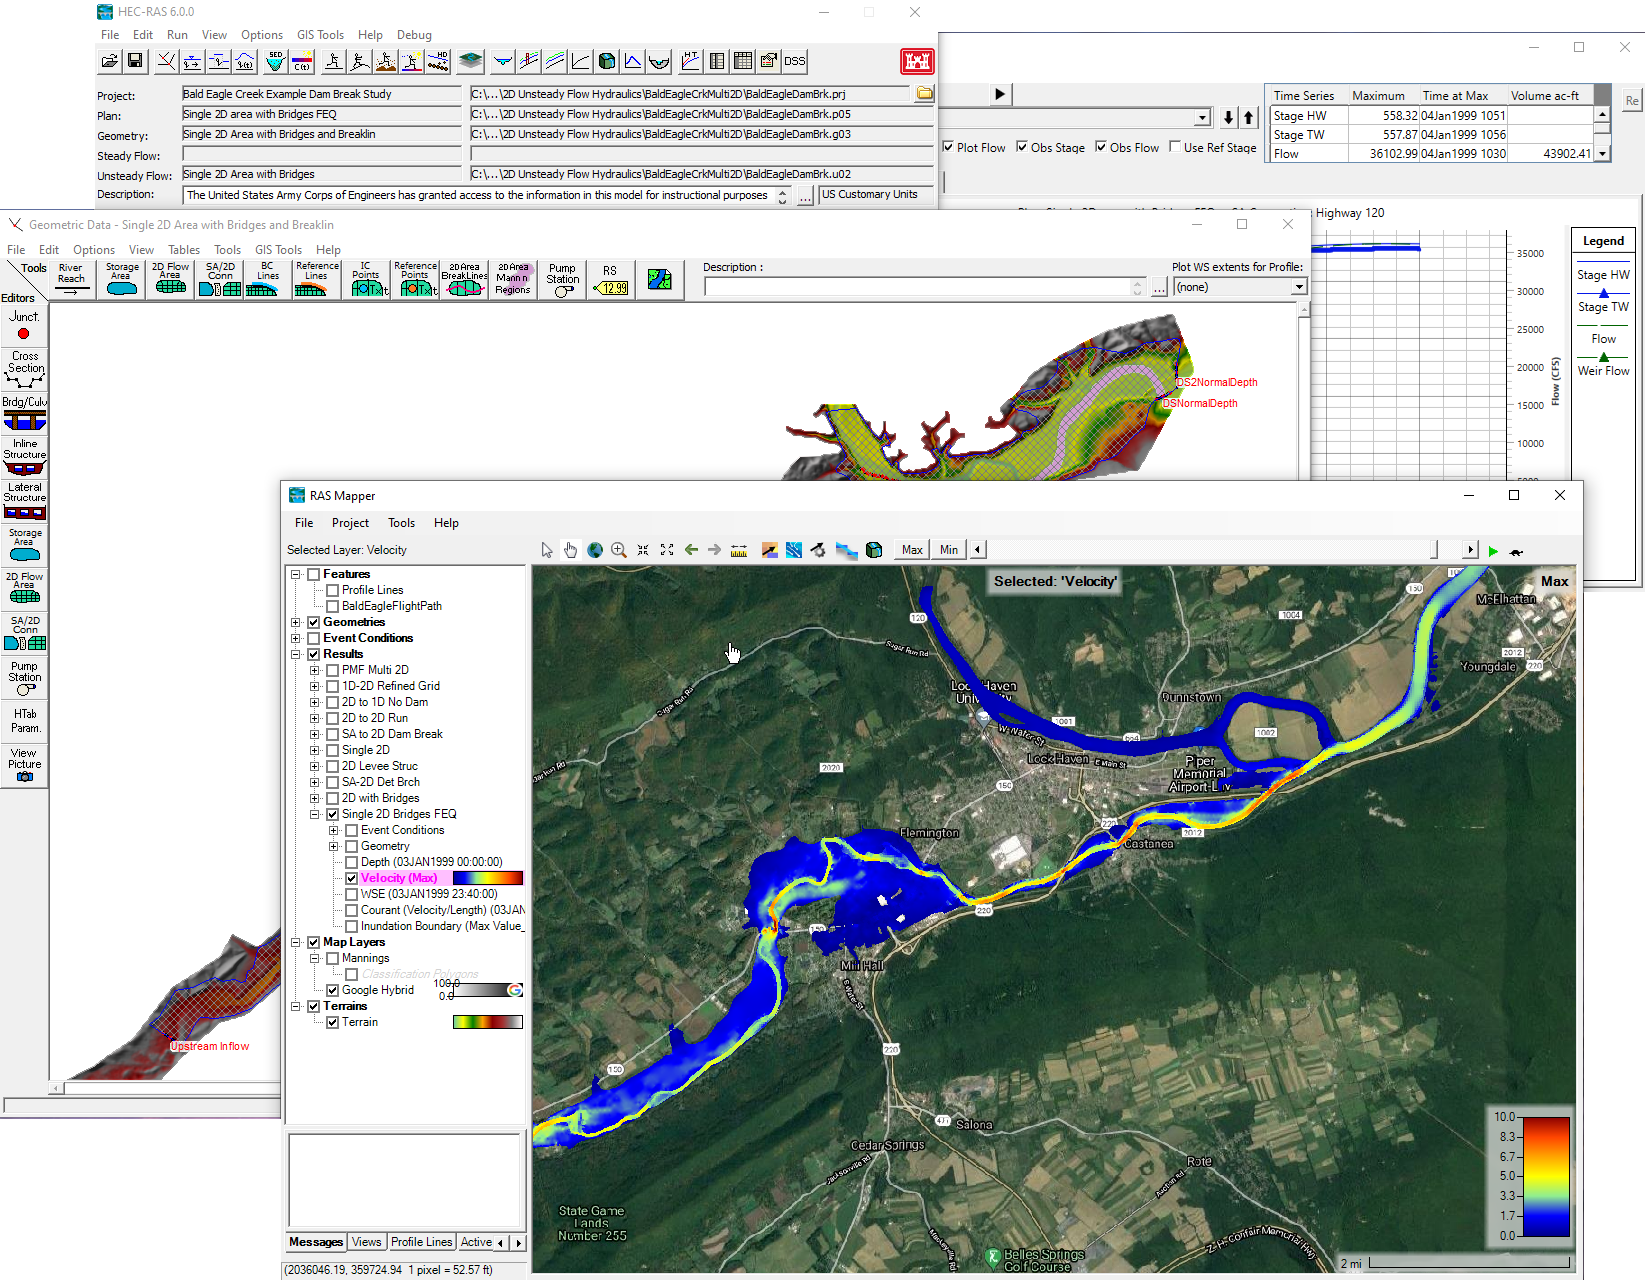
\includegraphics[width=\textwidth]{RAS-60}
\end{textblock*}
\end{frame}{}


\end{document}

